\documentclass[compress]{beamer}
\usepackage{irbookslide}
\usepackage{irilmenau2}
\usepackage{tikz}
\usepackage{url}
\usepackage{ifxetex}
%\RequireXeTeX
\usepackage{fontspec} % zahteva paket euenc
\usepackage{xunicode}
\usepackage{xltxtra}
\usepackage{polyglossia}
\usepackage{minted}
\usepackage[noend]{algorithmic}
\renewcommand{\algorithmicrequire}{\textbf{Input:}}
\renewcommand{\algorithmicensure}{\textbf{Output:}}
\renewcommand{\algorithmiccomment}[1]{\hfill \{\myred{#1}\}}
\usepackage{xcolor,colortbl}
\usepackage{textcomp}
\usepackage{unicode-math}
%\usepackage{hyphenat}
%\setdefaultlanguage[script=Latin]{serbian}

\title{Grafovi}
\author{\textcopyright \ \ Goodrich, Tamassia, Goldwasser}
\institute{Katedra za informatiku, Fakultet tehničkih nauka, Univerzitet u
Novom Sadu}
\date{2014.}
\subject{Predavanja sa ASP}

\begin{document}

\frame{\titlepage}

\section[Pojam]{Pojam grafa}

\begin{frame}[fragile]
  \frametitle{Pojam grafa}
  \begin{itemize}
    \item \myred{graf} je par $(V,E)$
    \begin{itemize}
      \item $V$ je set čvorova (\textit{vertices})
      \item $E$ je skup grana (\textit{edges})
      \item ćvorovi i grane čuvaju elemente
    \end{itemize}
    \item primer:
    \begin{itemize}
      \item čvorovi predstavljaju aerodrome i čuvaju šifre aerodroma
      \item grane predstavljaju letove između aerodroma i čuvaju dužinu puta
    \end{itemize}
  \end{itemize}
  \begin{center}
    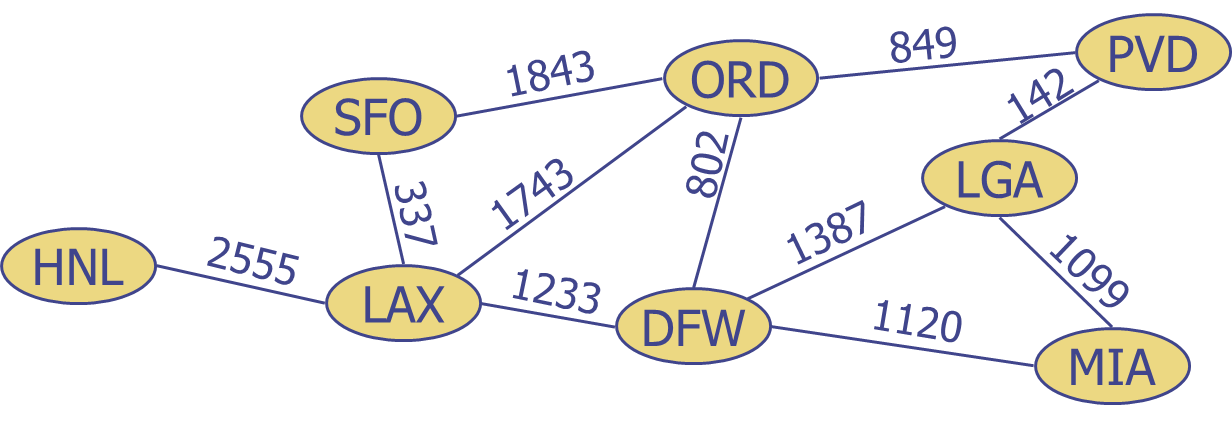
\includegraphics[width=10.5cm]{asp-14-pic01.png}
  \end{center}
\end{frame}

\begin{frame}[fragile]
  \frametitle{Vrste grana}
  \begin{columns}
    \begin{column}[t]{8cm}
      \begin{itemize}
        \item usmerena grana
        \begin{itemize}
          \item uređeni par čvorova $(u,v)$
          \item prvi čvor $u$ je polazište
          \item drugi čvor $v$ je odredište
          \item npr. konkretan let aviona
        \end{itemize}
        \item neusmerena grana
        \begin{itemize}
          \item neuređeni par čvorova $(u,v)$
          \item npr. putanja leta
        \end{itemize}
        \item usmereni graf
        \begin{itemize}
          \item sve grane su usmerene
          \item npr. mreža letova
        \end{itemize}
        \item neusmereni graf
        \begin{itemize}
          \item sve grane su neusmerene
          \item npr. mreža putanja
        \end{itemize}
      \end{itemize}
    \end{column}
    \begin{column}[t]{4cm}
      \begin{center}
        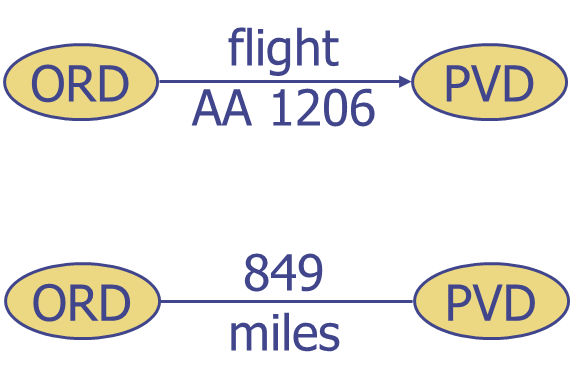
\includegraphics[width=4cm]{asp-14-pic02.png}
      \end{center}
    \end{column}
  \end{columns}
\end{frame}

\begin{frame}[fragile]
  \frametitle{Primene}
  \begin{columns}
    \begin{column}[t]{6cm}
      \begin{itemize}
        \item elektronska kola
        \begin{itemize}
          \item štampane ploče
          \item integrisana kola
        \end{itemize}
        \item transportne mreže
        \begin{itemize}
          \item putevi
          \item avionski letovi
        \end{itemize}
        \item računarske mreže
        \begin{itemize}
          \item lokalne mreže
          \item Internet
        \end{itemize}
        \item baze podataka
        \begin{itemize}
          \item ER dijagrami
        \end{itemize}
      \end{itemize}
    \end{column}
    \begin{column}[t]{6cm}
      \begin{center}
        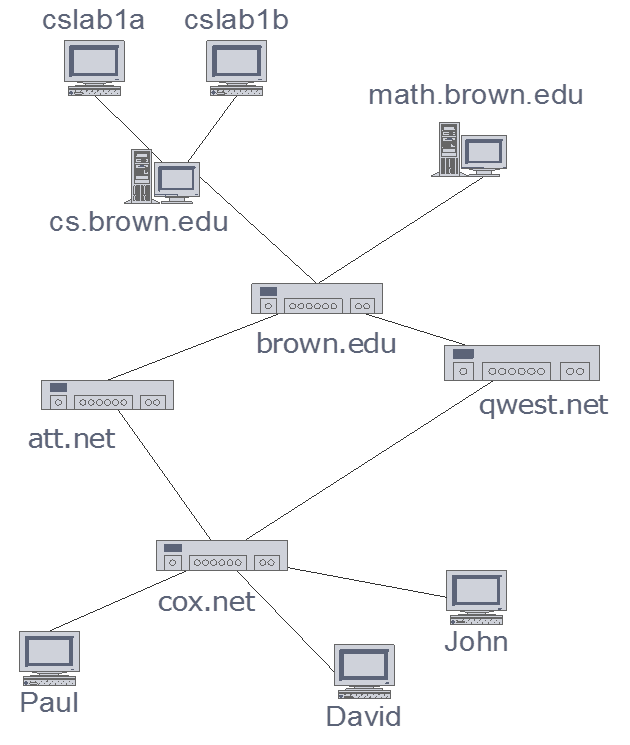
\includegraphics[width=6cm]{asp-14-pic03.png}
      \end{center}
    \end{column}
  \end{columns}
\end{frame}

\begin{frame}[fragile]
  \frametitle{Terminologija $_{1}$}
  \begin{columns}
    \begin{column}[t]{6cm}
      \begin{itemize}
        \item krajevi grane
        \begin{itemize}
          \item $U$ i $V$ su krajevi $a$
        \end{itemize}
        \item grane incidentne na čvoru
        \begin{itemize}
          \item $a$, $d$ i $b$ su incidentni na $V$
        \end{itemize}
        \item susedni čvorovi
        \begin{itemize}
          \item povezani granom
          \item $U$ i $V$ su susedni
        \end{itemize}
        \item stepen čvora
        \begin{itemize}
          \item broj grana kojima je on kraj
          \item stepen of $X$ je 5
        \end{itemize}
        \item paralelne grane: $h$ i $i$
        \item petlja: $j$
      \end{itemize}
    \end{column}
    \begin{column}[t]{6cm}
      \begin{center}
        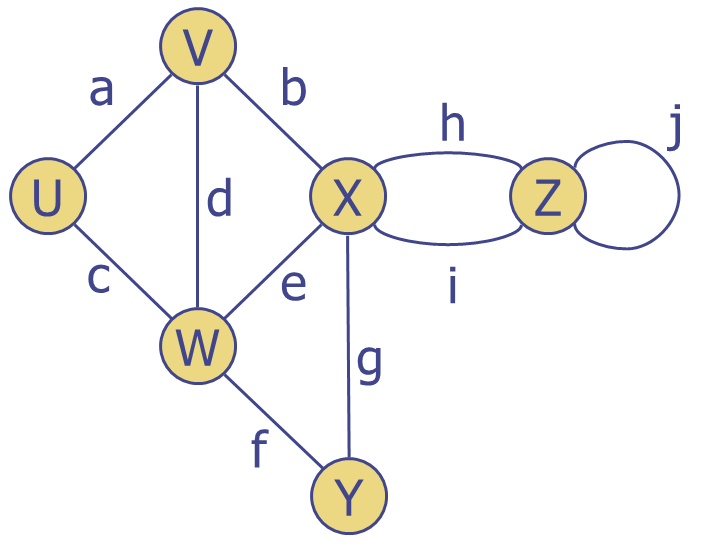
\includegraphics[width=6cm]{asp-14-pic04.png}
      \end{center}
    \end{column}
  \end{columns}
\end{frame}

\begin{frame}[fragile]
  \frametitle{Terminologija $_{2}$}
  \begin{columns}
    \begin{column}[t]{7.5cm}
      \begin{itemize}
        \item putanja
        \begin{itemize}
          \item sekvenca naizmenično čvorova i grana
          \item počinje sa čvorom
          \item završava sa čvorom
          \item svakoj grani prethodi i sledi njen kraj
        \end{itemize}
        \item prosta putanja
        \begin{itemize}
          \item svi čvorovi i grane su različiti
        \end{itemize}
        \item primeri
        \begin{itemize}
          \item $P_{1}=(V,b,X,h,Z)$ je prosta
          \item $P_{2}=(U,c,W,e,X,g,Y,f,W,d,V)$ nije prosta
        \end{itemize}
      \end{itemize}
    \end{column}
    \begin{column}[t]{4.5cm}
      \begin{center}
        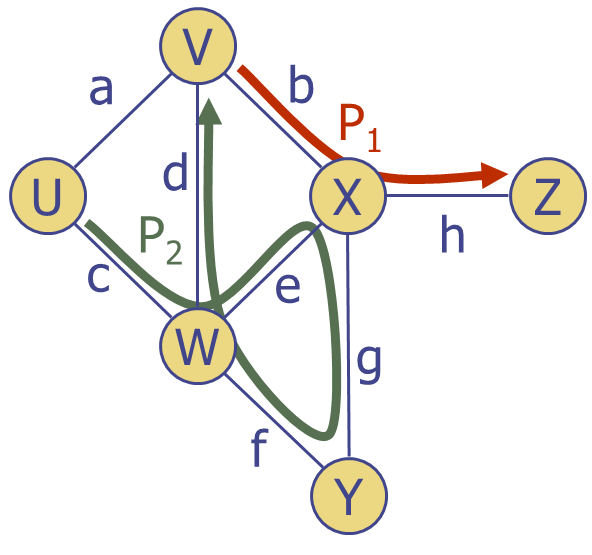
\includegraphics[width=4.5cm]{asp-14-pic05.png}
      \end{center}
    \end{column}
  \end{columns}
\end{frame}

\begin{frame}[fragile]
  \frametitle{Terminologija $_{3}$}
  \begin{columns}
    \begin{column}[t]{7.5cm}
      \begin{itemize}
        \item petlja
        \begin{itemize}
          \item cirkularna sekvenca naizmenično čvorova i grana
          \item svakoj grani prethodi i sledi njen kraj
        \end{itemize}
        \item prosta petlja
        \begin{itemize}
          \item s vi čvorovi i grane su različiti
        \end{itemize}
        \item primeri
        \begin{itemize}
          \item $C_{1}=(V,b,X,g,Y,f,W,c,U,a,V)$ je prosta
          \item $C_{2}=(U,c,W,e,X,g,Y,f,W,d,V,a,U)$ nije prosta
        \end{itemize}
      \end{itemize}
    \end{column}
    \begin{column}[t]{4.5cm}
      \begin{center}
        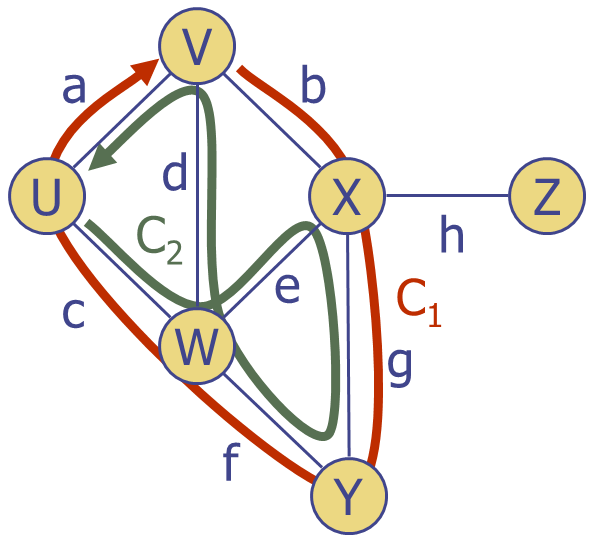
\includegraphics[width=4.5cm]{asp-14-pic06.png}
      \end{center}
    \end{column}
  \end{columns}
\end{frame}

\begin{frame}[fragile]
  \frametitle{Osobine}
  \begin{columns}
    \begin{column}[t]{7.5cm}
      \begin{itemize}
        \item suma stepena čvorova
        $$\sum_{v}deg(v)=2m$$ 
        \item u neusmerenom grafu bez petlji i 
        \begin{itemize}
          \item s vi čvorovi i grane su različiti
        \end{itemize}
        \item primeri
        \begin{itemize}
          \item $C_{1}=(V,b,X,g,Y,f,W,c,U,a,V)$ je prosta
          \item $C_{2}=(U,c,W,e,X,g,Y,f,W,d,V,a,U)$ nije prosta
        \end{itemize}
      \end{itemize}
    \end{column}
    \begin{column}[t]{4.5cm}
      \begin{center}
        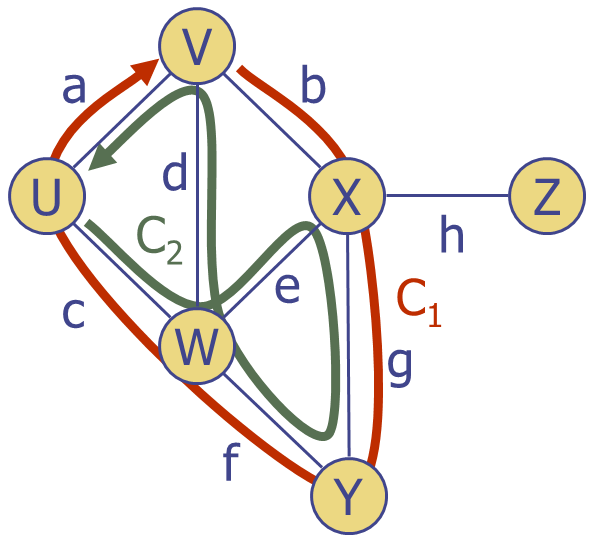
\includegraphics[width=4.5cm]{asp-14-pic06.png}
      \end{center}
    \end{column}
  \end{columns}
\end{frame}

\begin{frame}[fragile]
  \frametitle{Ćvorovi i grane}
  \begin{itemize}
    \item graf je kolekcija čvorova i grana
    \item prikazaćemo ga pomoću tri tipa: \texttt{Vertex}, \texttt{Edge} 
    i \texttt{Graph}
    \item \texttt{Vertex} je ,,lagani`` objekat koji čuva sadržaj (npr.
    šifru aerodroma)
    \begin{itemize}
      \item ima metodu \texttt{element()} kojom se može dobiti taj sadržaj
    \end{itemize}
    \item \texttt{Edge} čuva sadržaj (npr. broj leta, rastojanje)
    \begin{itemize}
      \item \texttt{element()} vraća taj sadržaj
      \item \texttt{endpoints()} vraća par $(u,v)$ polazište i odredište
      \item \texttt{opposite(v)} vraća suprotni kraj grane
    \end{itemize}
  \end{itemize}
\end{frame}

\begin{frame}[fragile]
  \frametitle{Graf ATP}
  {\scriptsize
  \begin{tabular}{r|p{6cm}}
    \texttt{vertex\_count()} & broj čvorova \\ \hline
    \texttt{vertices()} & lista svih čvorova \\ \hline
    \texttt{edge\_count()} & broj grana \\ \hline
    \texttt{edges()} & lista svih grana \\ \hline
    \texttt{get\_edge(u,v)} & vraća granu između \texttt{u} i \texttt{v}
      ako postoji, inače \texttt{None} \\ \hline
    \texttt{degree(v,out=True)} & broj izlaznih/ulaznih grana iz 
      \texttt{v} \\ \hline
    \texttt{incident\_edges(v,out=True)} & lista izlaznih/ulaznih grana 
      iz \texttt{v} \\ \hline
    \texttt{insert\_vertex(x=None)} & dodaj novi čvor sa sadržajem 
      \texttt{x} \\ \hline
    \texttt{insert\_edge(u,v,x=None)} & dodaj novu granu od \texttt{u} 
      ka \texttt{v} sa sadržajem \texttt{x}\\ \hline
    \texttt{remove\_vertex(v)} & ukloni čvor \texttt{v} i sve vezane 
      grane \\ \hline
    \texttt{remove\_edge(e)} & ukloni granu \texttt{e} \\
  \end{tabular}
  }
\end{frame}

\begin{frame}[fragile]
  \frametitle{Lista čvorova i lista grana}
  \begin{columns}
    \begin{column}[t]{6cm}
      \begin{itemize}
        \item \texttt{Vertex}
        \begin{itemize}
          \item čuva sadržaj
          \item element liste
        \end{itemize}
        \item \texttt{Edge}
        \begin{itemize}
          \item čuva sadržaj
          \item referenca na polazište
          \item referenca na odredište
          \item element liste
        \end{itemize}
        \item lista čvorova
        \item lista grana
      \end{itemize}
    \end{column}
    \begin{column}[t]{6cm}
      \begin{center}
        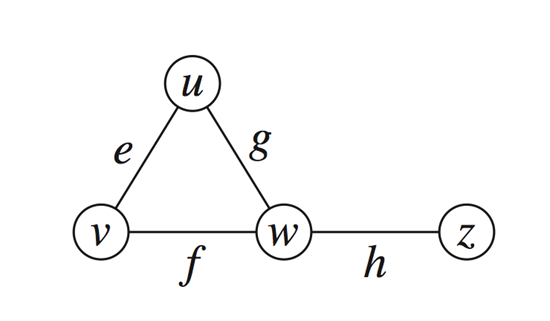
\includegraphics[width=4cm]{asp-14-pic08.png} \\
        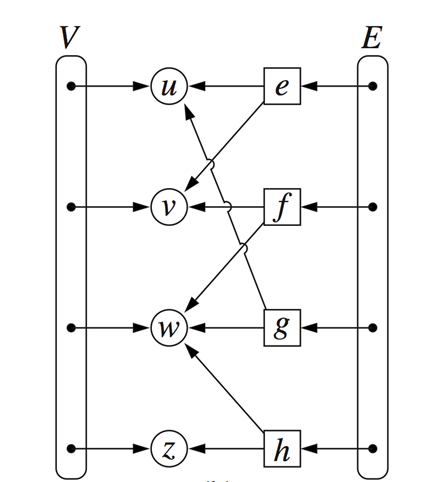
\includegraphics[width=4cm]{asp-14-pic09.png}
      \end{center}
    \end{column}
  \end{columns}
\end{frame}

\begin{frame}[fragile]
  \frametitle{Lista suseda}
  \begin{columns}
    \begin{column}[t]{6cm}
      \begin{itemize}
        \item lista grana za svaki čvor
        \item grane mogu imati reference na drugu pojavu iste grane (za 
          drugi krajnji čvor)
      \end{itemize}
    \end{column}
    \begin{column}[t]{6cm}
      \begin{center}
        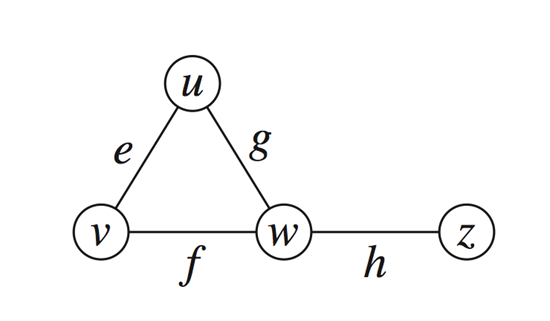
\includegraphics[width=4cm]{asp-14-pic10.png} \\
        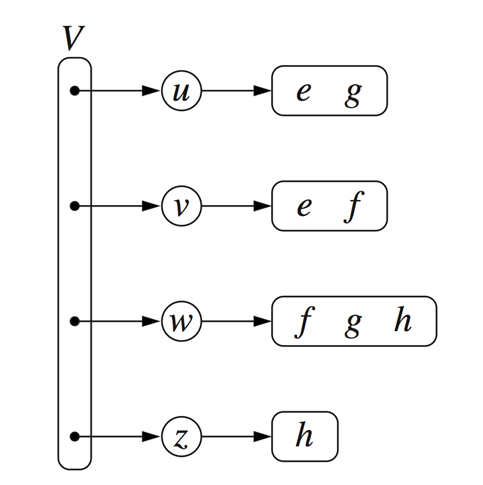
\includegraphics[width=4cm]{asp-14-pic11.png}
      \end{center}
    \end{column}
  \end{columns}
\end{frame}

\begin{frame}[fragile]
  \frametitle{Matrica incidencije}
  \begin{columns}
    \begin{column}[t]{6cm}
      \begin{itemize}
        \item svakom čvoru dodeljen int ključ
        \item matrica sadrži referencu na granu ukoliko ona povezuje
          dva čvora, ili None
        \item ili samo 0/1 u matrici
      \end{itemize}
    \end{column}
    \begin{column}[t]{6cm}
      \begin{center}
        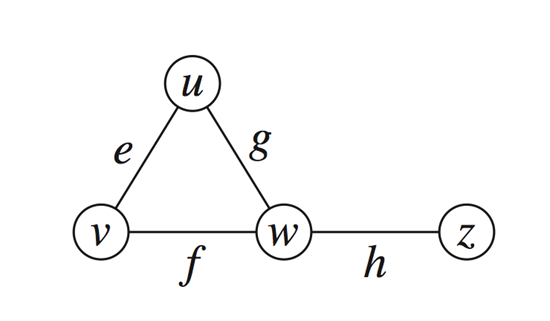
\includegraphics[width=5cm]{asp-14-pic12.png} \\
        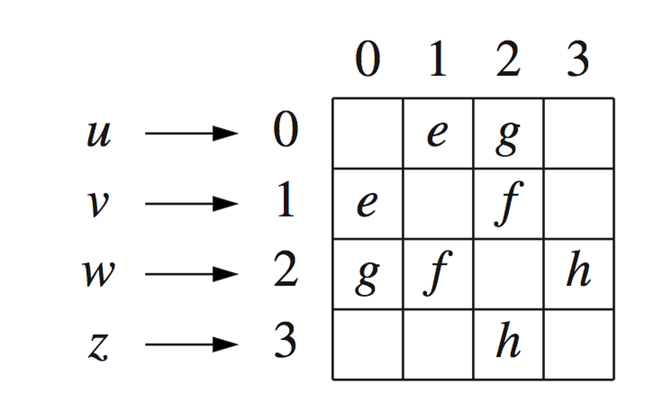
\includegraphics[width=5cm]{asp-14-pic13.png}
      \end{center}
    \end{column}
  \end{columns}
\end{frame}

\begin{frame}[fragile]
  \frametitle{Performanse}
  %\begin{itemize}
    %\item 
    $n$ čvorova, $m$ grana, bez paralelnih grana, bez petlji \\ \ \\
  %\end{itemize}
  %{\scriptsize
  \begin{tabular}{l|c|c|c}
     & lista & lista & matrica \\
     & grana & suseda & incidencije \\ \hline     
    \textit{prostor} & $n+m$ & $n+m$ & $n^2$ \\ \hline
    \texttt{incident\_edges(v)} & $m$ & $deg(v)$ & $n$ \\ \hline
    \texttt{are\_adjacent(v,w)} & $m$ & $\min\{deg(v),deg(w)\}$ & $1$ \\ \hline
    \texttt{insert\_vertex(v)} & $1$ & $1$ & $n^2$ \\ \hline
    \texttt{insert\_edge(v,w,e)} & $1$ & $1$ & $1$ \\ \hline
    \texttt{remove\_vertex(v)} & $m$ & $deg(v)$ & $n^2$ \\ \hline
    \texttt{remove\_edge(e)} & $1$ & $1$ & $1$ \\
  \end{tabular}
  %}
\end{frame}

\begin{frame}[fragile]
  \frametitle{Python implementacija}
  \begin{itemize}
    \item koristićemo mapu susedstva
    \item za čvor $v$ čuvamo Python rečnik sa susedima $I(v)$
    \item listu čvorova zamenićemo rečnikom $D$ koji mapira svaki čvor 
      na njegovu mapu suseda $I(v)$
    \begin{itemize}
      \item možemo proći kroz sve čvorove sa \texttt{D.keys()}
    \end{itemize}
    \item čvor ne mora da čuva svoj položaj u $D$ jer se to izračuna za 
      $O(1)$
    \item performanse iste kao za listu suseda ali u \textbf{očekivanom}
      slučaju
  \end{itemize}
\end{frame}

\begin{frame}[fragile,shrink]
  \frametitle{Klasa Vertex}
\begin{minted}[linenos=false]{python}
class Vertex:
  """Lightweight vertex structure for a graph."""
  __slots__ = '_element'

  def __init__(self, x):
    """Do not call constructor directly. 
    Use Graph's insert_vertex(x).
    """
    self._element = x

  def element(self):
    """Return element associated with this vertex."""
    return self._element

  def __hash__(self):  # will allow vertex to be a map/set key
    return hash(id(self))

  def __str__(self):
    return str(self._element)
\end{minted}
\end{frame}

\begin{frame}[fragile,shrink]
  \frametitle{Klasa Edge}
\begin{minted}[linenos=false]{python}
class Edge:
  __slots__ = '_origin', '_destination', '_element'

  def __init__(self, u, v, x):
    self._origin = u
    self._destination = v
    self._element = x

  def endpoints(self):
    return (self._origin, self._destination)

  def opposite(self, v):
    if not isinstance(v, Graph.Vertex):
      raise TypeError('v must be a Vertex')
    return self._destination if v is self._origin else self._origin
    raise ValueError('v not incident to edge')

  def element(self):
    return self._element

  def __hash__(self):  # will allow edge to be a map/set key
    return hash( (self._origin, self._destination) )

  def __str__(self):
    return '({0},{1},{2})'.format(self._origin,self._destination,self._element)
\end{minted}
\end{frame}

\begin{frame}[fragile,shrink]
  \frametitle{Klasa Graph $_1$}
\begin{minted}[linenos=false]{python}
class Graph:
  def __init__(self, directed=False):
    self._outgoing = {}
    self._incoming = {} if directed else self._outgoing

  def _validate_vertex(self, v):
    if not isinstance(v, self.Vertex):
      raise TypeError('Vertex expected')
    if v not in self._outgoing:
      raise ValueError('Vertex does not belong to this graph.')
    
  def is_directed(self):
    return self._incoming is not self._outgoing

  def vertex_count(self):
    return len(self._outgoing)

  def vertices(self):
    return self._outgoing.keys()
\end{minted}
\end{frame}

\begin{frame}[fragile,shrink]
  \frametitle{Klasa Graph $_2$}
\begin{minted}[linenos=false]{python}
  def edge_count(self):
    total = sum(len(self._outgoing[v]) for v in self._outgoing)
    return total if self.is_directed() else total // 2

  def edges(self):
    result = set() # avoid double-reporting edges of undirected graph
    for secondary_map in self._outgoing.values():
      result.update(secondary_map.values()) # add edges to resulting set
    return result

  def get_edge(self, u, v):
    self._validate_vertex(u)
    self._validate_vertex(v)
    return self._outgoing[u].get(v) # returns None if v not adjacent

  def degree(self, v, outgoing=True):   
    self._validate_vertex(v)
    adj = self._outgoing if outgoing else self._incoming
    return len(adj[v])
\end{minted}
\end{frame}

\begin{frame}[fragile,shrink]
  \frametitle{Klasa Graph $_3$}
\begin{minted}[linenos=false]{python}
  def incident_edges(self, v, outgoing=True):   
    self._validate_vertex(v)
    adj = self._outgoing if outgoing else self._incoming
    for edge in adj[v].values():
      yield edge

  def insert_vertex(self, x=None):
    v = self.Vertex(x)
    self._outgoing[v] = {}
    if self.is_directed():
      self._incoming[v] = {} # need distinct map for incoming edges
    return v
      
  def insert_edge(self, u, v, x=None):
    if self.get_edge(u, v) is not None:  # includes error checking
      raise ValueError('u and v are already adjacent')
    e = self.Edge(u, v, x)
    self._outgoing[u][v] = e
    self._incoming[v][u] = e
\end{minted}
\end{frame}

\begin{frame}[fragile]
  \frametitle{Podgraf}
  \begin{columns}
    \begin{column}[t]{6cm}
      \begin{itemize}
        \item \myred{podgraf} $S$ grafa $G$ je graf takav da
        \begin{itemize}
          \item čvorovi $S$ su podskup čvorova $G$
          \item grane $S$ su podskup grana $G$ \\ \ \\
        \end{itemize}
        \item \myred{pokrivajući podgraf} sadrži sve čvorove $G$
      \end{itemize}
    \end{column}
    \begin{column}[t]{6cm}
      \begin{center}
        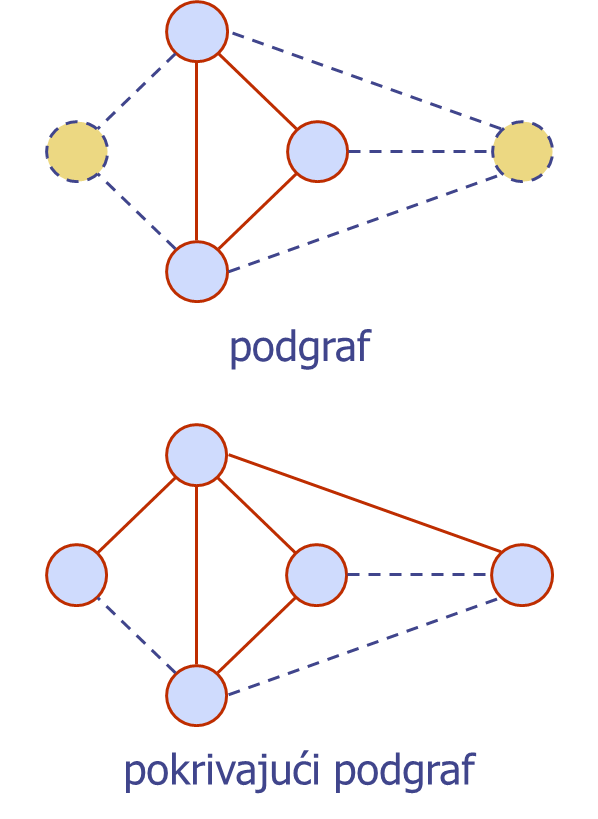
\includegraphics[width=5cm]{asp-14-pic14.png}
      \end{center}
    \end{column}
  \end{columns}
\end{frame}

\begin{frame}[fragile]
  \frametitle{Povezanost}
  \begin{columns}
    \begin{column}[t]{6cm}
      \begin{itemize}
        \item graf je \myred{povezan} ako postoji putanja između svaka 
          dva čvora
        \item \myred{povezana komponenta} je maksimalni povezani podgraf
      \end{itemize}
    \end{column}
    \begin{column}[t]{6cm}
      \begin{center}
        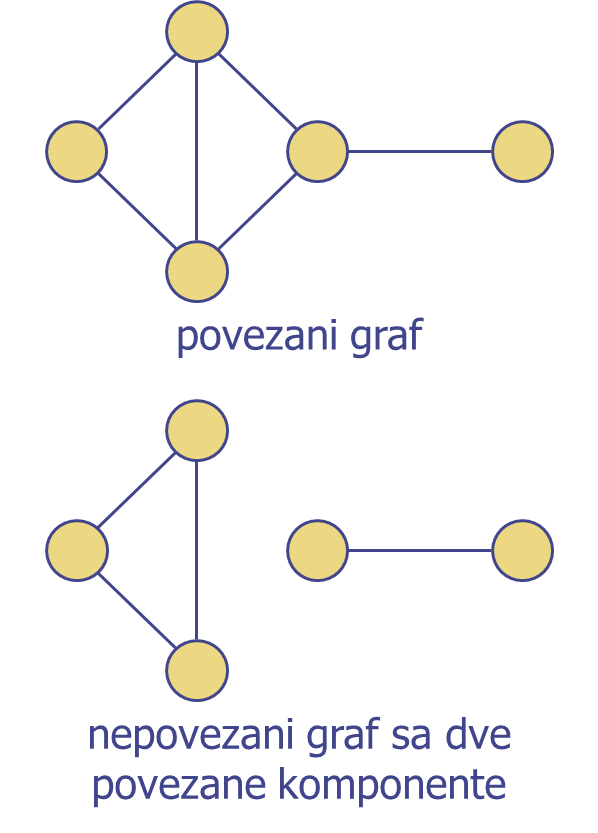
\includegraphics[width=5cm]{asp-14-pic15.png}
      \end{center}
    \end{column}
  \end{columns}
\end{frame}

\begin{frame}[fragile]
  \frametitle{Stablo i šuma}
  \begin{columns}
    \begin{column}[t]{6cm}
      \begin{itemize}
        \item \myred{stablo} je neusmereni graf $T$ takav da
        \begin{itemize}
          \item $T$ je povezan
          \item $T$ nema petlje
        \end{itemize}
        \item \myred{šuma} je neusmereni graf takav da
        \begin{itemize}
          \item nema petlje
          \item povezane komponente su stabla
        \end{itemize}
      \end{itemize}
    \end{column}
    \begin{column}[t]{6cm}
      \begin{center}
        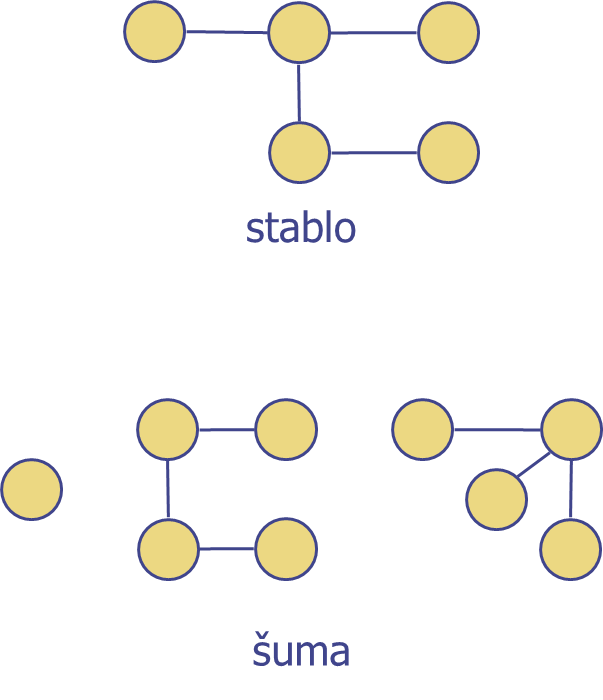
\includegraphics[width=5cm]{asp-14-pic16.png}
      \end{center}
    \end{column}
  \end{columns}
\end{frame}

\begin{frame}[fragile]
  \frametitle{Pokrivajuće stablo i šuma}
  \begin{columns}
    \begin{column}[t]{6cm}
      \begin{itemize}
        \item \myred{pokrivajuće stablo} je podgraf koji
        \begin{itemize}
          \item je stablo i
          \item pokriva graf
        \end{itemize}
        \item pokrivajuće stablo nije jedinstveno ako graf nije stablo
        \item \myred{pokrivajuća šuma} je podgraf koji
        \begin{itemize}
          \item je šuma i
          \item pokriva graf
        \end{itemize}
      \end{itemize}
    \end{column}
    \begin{column}[t]{6cm}
      \begin{center}
        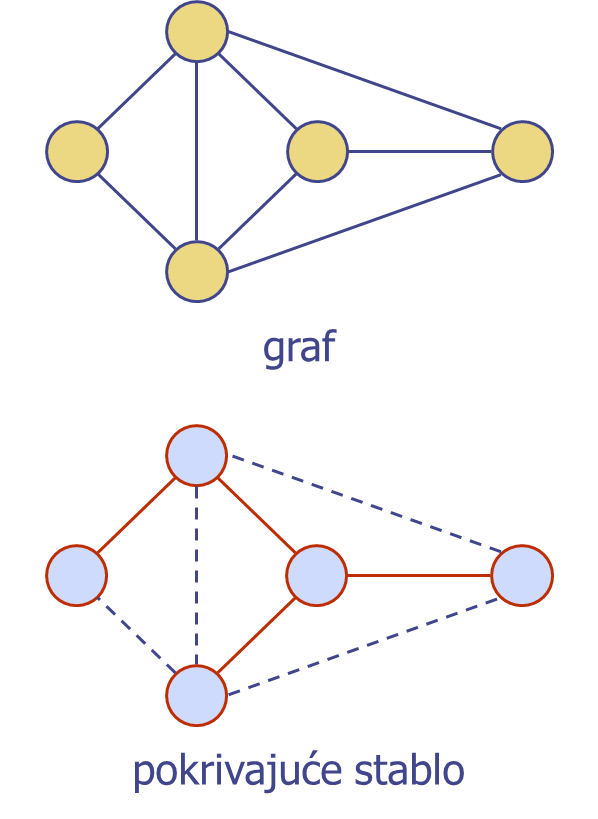
\includegraphics[width=5cm]{asp-14-pic17.png}
      \end{center}
    \end{column}
  \end{columns}
\end{frame}

\section[Obilazak]{Obilazak grafa}

\begin{frame}[fragile]
  \frametitle{Obilazak grafa po dubini}
  \begin{columns}
    \begin{column}[t]{6cm}
      \begin{itemize}
        \item depth-first-search (\myred{DFS}) je opšti metod za 
        obilazak grafa
        \begin{itemize}
          \item obilazi sve čvorove i grane
          \item određuje da li je graf povezan
          \item određuje povezane komponente grafa
          \item određuje pokrivajuću šumu grafa
        \end{itemize}
      \end{itemize}
    \end{column}
    \begin{column}[t]{6cm}
      \begin{itemize}
        \item DFS na grafu sa $n$ čvorova i $m$ grana traje $O(n+m)$
        \item može se proširiti za rešavanje drugih problema
        \begin{itemize}
          \item nađi putanju između dva čvora
          \item nađi petlju u grafu
        \end{itemize}
        \item DFS je za graf isto što i Ojlerov obilazak za binarna 
          stabla
      \end{itemize}
    \end{column}
  \end{columns}
\end{frame}

\begin{frame}[fragile]
  \frametitle{DFS algoritam}
  dodeljuje oznake (labele) čvorovima i granama
  {\footnotesize
  \begin{columns}
    \begin{column}[t]{6cm}
      \myred{DFS}($G$)
      \begin{algorithmic}
        \REQUIRE graf $G$
        \ENSURE oznake na granama: {\scriptsize DISCOVERY} ili {\scriptsize BACK}
        \FORALL{$u\in G$.vertices()}
          \STATE setLabel($u$, {\scriptsize UNEXPLORED})
        \ENDFOR
        \FORALL{$e\in G$.edges()}
          \STATE setLabel($e$, {\scriptsize UNEXPLORED})
        \ENDFOR
        \FORALL{$v\in G$.vertices()}
          \IF{label($v$) = {\scriptsize UNEXPLORED}}
            \STATE DFS($G,v$)
          \ENDIF
        \ENDFOR
      \end{algorithmic}
    \end{column}
    \begin{column}[t]{6cm}
      \myred{DFS}($G,v$)
      \begin{algorithmic}
        \REQUIRE graf $G$ i početni čvor $v$
        \ENSURE oznake na granama: {\scriptsize DISCOVERY} ili {\scriptsize BACK}
        \STATE setLabel($v$, {\scriptsize VISITED})
        \FORALL{$e\in G$.incidentEdges($v$)}
          \IF{label($e$) = {\scriptsize UNEXPLORED}}
            \STATE $w \leftarrow$ opposite($v,e$)
            \IF{label($e$) = {\scriptsize UNEXPLORED}}
              \STATE setLabel($e$, {\scriptsize DISCOVERY})
              \STATE DFS($G, w$)
            \ELSE
              \STATE setLabel($e$, {\scriptsize BACK})
            \ENDIF
          \ENDIF
        \ENDFOR
      \end{algorithmic}
    \end{column}
  \end{columns}
  }
\end{frame}

\begin{frame}[fragile,shrink=15]
  \frametitle{DFS u Pythonu}
\begin{minted}[linenos=false]{python}
def DFS(g, u, discovered):
  for e in g.incident_edges(u): # for every outgoing edge from u
    v = e.opposite(u)
    if v not in discovered:  # v is an unvisited vertex
      discovered[v] = e      # e is the tree edge that discovered v
      DFS(g, v, discovered)  # recursively explore from v
\end{minted}
\end{frame}

\begin{frame}[fragile]
  \frametitle{DFS primer}
  \begin{center}
    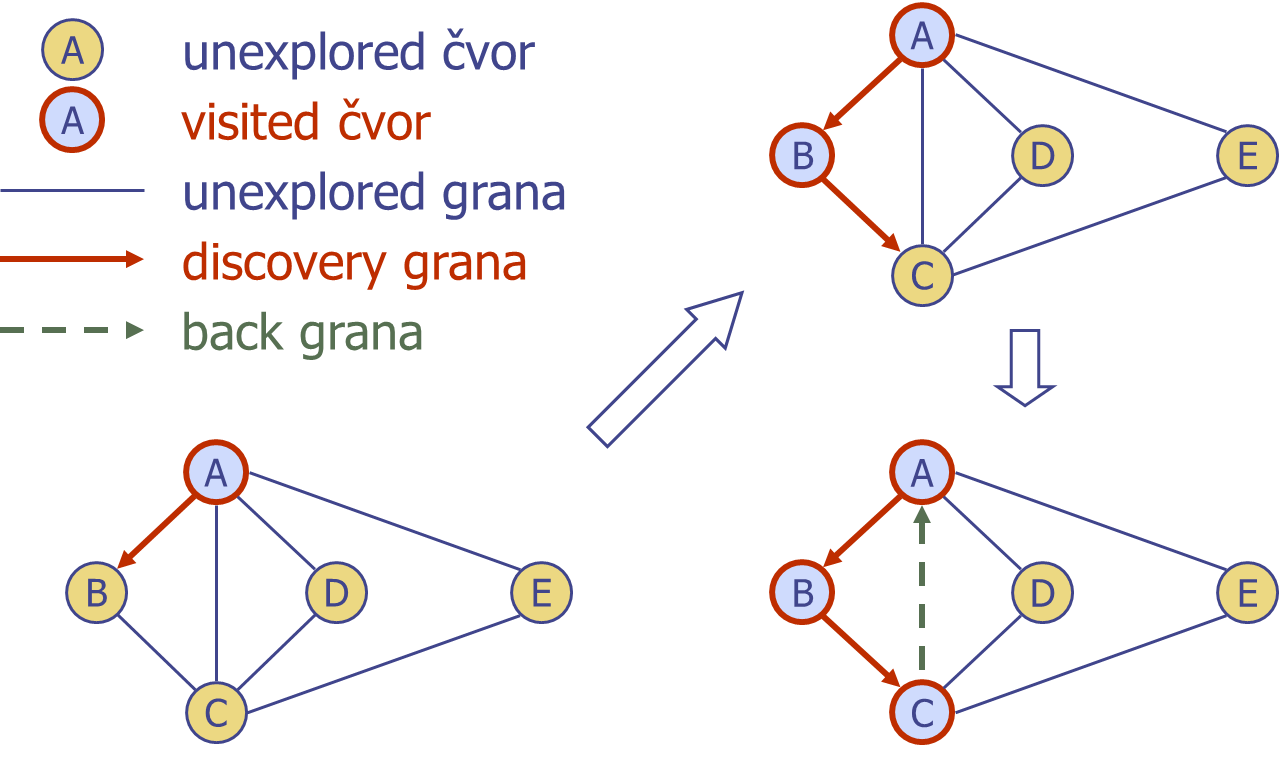
\includegraphics[width=11cm]{asp-14-pic18.png}
  \end{center}
\end{frame}

\begin{frame}[fragile]
  \frametitle{DFS primer (još)}
  \begin{center}
    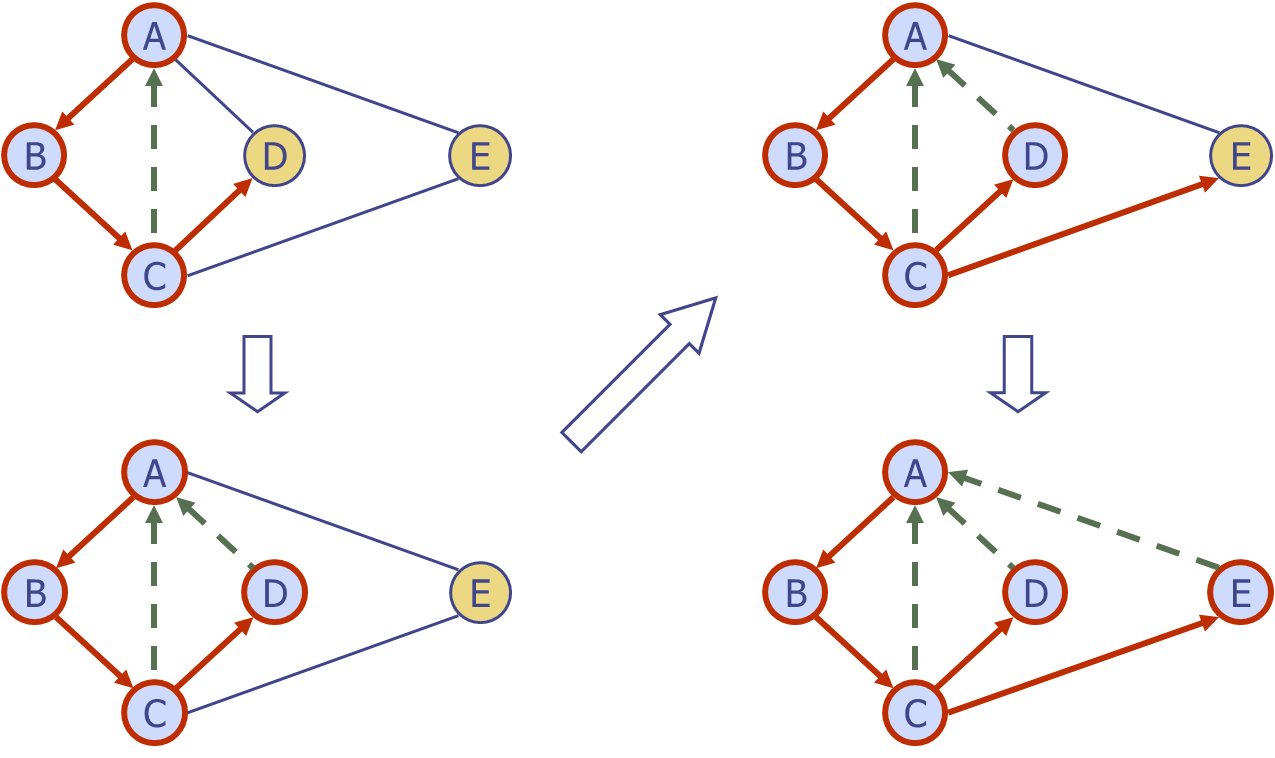
\includegraphics[width=11cm]{asp-14-pic19.png}
  \end{center}
\end{frame}

\begin{frame}[fragile]
  \frametitle{DFS i prolazak lavirinta}
  \begin{columns}
    \begin{column}[t]{6cm}
      \begin{itemize}
        \item svaku raskrsnicu, ugao (skretanje) i kraj puta označimo
          kao posećen čvor
        \item svaki hodnik (granu) kao posećenu
        \item pamtimo odakle smo počeli pomoću steka rekurzije
      \end{itemize}
    \end{column}
    \begin{column}[t]{6cm}
      \begin{center}
        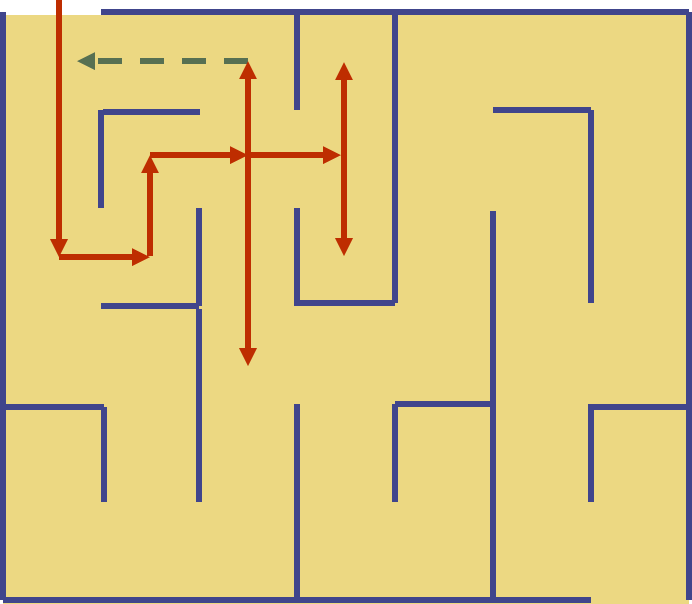
\includegraphics[width=6cm]{asp-14-pic20.png}
      \end{center}
    \end{column}
  \end{columns}
\end{frame}

\begin{frame}[fragile]
  \frametitle{Osobine DFS}
  \begin{columns}
    \begin{column}[t]{6cm}
      \begin{itemize}
        \item[1] DFS($G,v$) obilazi sve čvorove i grane u povezanoj 
          komponenti od $v$
        \item[2] grane označene kao {\scriptsize DISCOVERY} čine 
          pokrivajuće stablo povezane komponente od $v$
      \end{itemize}
    \end{column}
    \begin{column}[t]{6cm}
      \begin{center}
        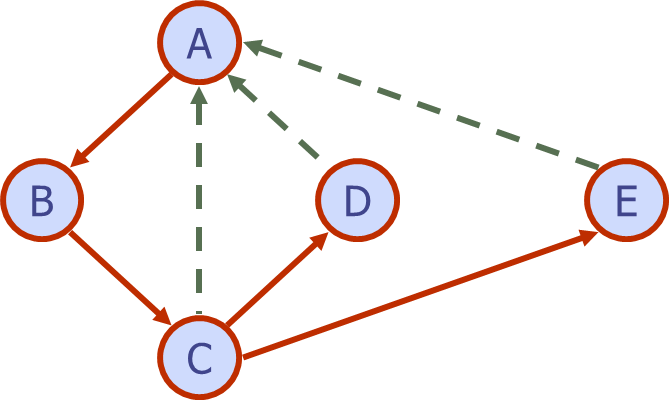
\includegraphics[width=5cm]{asp-14-pic21.png}
      \end{center}
    \end{column}
  \end{columns}
\end{frame}

\begin{frame}[fragile]
  \frametitle{Performanse DFS}
  \begin{itemize}
    \item stavljanje labele na čvor/granu traje $O(1)$
    \item svaki čvor se označi \textbf{dva} puta, jednom kao {\scriptsize 
      UNEXPLORED}, drugi put kao {\scriptsize VISITED}
    \item svaka grana se označi \textbf{dva} puta, jednom kao {\scriptsize 
      UNEXPLORED}, drugi put kao {\scriptsize DISCOVERY} ili 
      {\scriptsize BACK}
    \item metoda \texttt{incident\_edges} se poziva jednom za svaki čvor
    \item DFS traje $O(n+m)$ ako je graf predstavljen listom suseda
    $$\sum_{v}deg(v)=2m$$
  \end{itemize}
\end{frame}

\begin{frame}[fragile]
  \frametitle{DFS za pronalaženje putanje}
  {\footnotesize
  \begin{columns}
    \begin{column}[t]{6cm}
      \begin{itemize}
        \item DFS se može upotrebiti za pronalaženje putanje između dva
          čvora $u$ i $z$
        \item pozivamo DFS($G,u$) sa $u$ kao početnim čvorom
        \item na steku $S$ čuvamo putanju od početnog do tekućeg čvora
        \item kada dođemo do $z$ na steku je cela putanja
      \end{itemize}
    \end{column}
    \begin{column}[t]{6cm}
      \myred{DFS}($G,v$)
      \begin{algorithmic}
        \REQUIRE graf $G$ i početni čvor $v$
        \ENSURE oznake na granama: {\scriptsize DISCOVERY} ili {\scriptsize BACK}
        \STATE setLabel($v$, {\scriptsize VISITED})
        \FORALL{$e\in G$.incidentEdges($v$)}
          \IF{label($e$) = {\scriptsize UNEXPLORED}}
            \STATE $w \leftarrow$ opposite($v,e$)
            \IF{label($e$) = {\scriptsize UNEXPLORED}}
              \STATE setLabel($e$, {\scriptsize DISCOVERY})
              \STATE DFS($G, w$)
            \ELSE
              \STATE setLabel($e$, {\scriptsize BACK})
            \ENDIF
          \ENDIF
        \ENDFOR
      \end{algorithmic}
    \end{column}
  \end{columns}
  }
\end{frame}

\end{document}
